% Template for Cogsci submission with R Markdown

% Stuff changed from original Markdown PLOS Template
\documentclass[10pt, letterpaper]{article}

\usepackage{cogsci}
\usepackage{pslatex}
\usepackage{float}
\usepackage{caption}

% amsmath package, useful for mathematical formulas
\usepackage{amsmath}

% amssymb package, useful for mathematical symbols
\usepackage{amssymb}

% hyperref package, useful for hyperlinks
\usepackage{hyperref}

% graphicx package, useful for including eps and pdf graphics
% include graphics with the command \includegraphics
\usepackage{graphicx}

% Sweave(-like)
\usepackage{fancyvrb}
\DefineVerbatimEnvironment{Sinput}{Verbatim}{fontshape=sl}
\DefineVerbatimEnvironment{Soutput}{Verbatim}{}
\DefineVerbatimEnvironment{Scode}{Verbatim}{fontshape=sl}
\newenvironment{Schunk}{}{}
\DefineVerbatimEnvironment{Code}{Verbatim}{}
\DefineVerbatimEnvironment{CodeInput}{Verbatim}{fontshape=sl}
\DefineVerbatimEnvironment{CodeOutput}{Verbatim}{}
\newenvironment{CodeChunk}{}{}

% cite package, to clean up citations in the main text. Do not remove.
\usepackage{apacite}

% KM added 1/4/18 to allow control of blind submission
\cogscifinalcopy

\usepackage{color}

% Use doublespacing - comment out for single spacing
%\usepackage{setspace}
%\doublespacing


% % Text layout
% \topmargin 0.0cm
% \oddsidemargin 0.5cm
% \evensidemargin 0.5cm
% \textwidth 16cm
% \textheight 21cm

\title{Using pretense behavior to explore counterfactual
self-simulation}


\author{{\large \bf Matan Mazor (mtnmzor@gmail.com)} \\ Birkbeck, University of london \\ London, WC1E 7HX UK \AND {\large \bf Chaz Firestone (chaz@jhu.edu)} \AND {\large \bf Ian Phillips (ianphillips@jhu.edu)} \\ Johns Hopkins University \\ Baltimore, MD 21218, USA}

\newlength{\cslhangindent}
\setlength{\cslhangindent}{1.5em}
\newenvironment{CSLReferences}%
  {}%
  {\par}

\begin{document}

\maketitle

\begin{abstract}
What we do depends on what we know. But sometimes we try to decouple our
behavior from our knowledge so that we appear not to know what we really
do know. Such pretense behavior requires understanding how we would
behave with different knowledge --- and so provides a window into
counterfactual self-simulation. However, little research has
characterized and evaluated pretense relative to non-pretense behavior.
Here, in a large-scale, pre-registered experiment, subjects played
normal games of Battleships (trying to sink ships hidden in a grid), as
well as `pretend' games, where they were told all the ships' locations
but had to pretend they were playing normally. Relative to normal games,
`pretend' games demonstrated similar but exaggerated behavioral
patterns. Furthermore, pretenders played rationally, but less so than
non-pretenders. Despite these differences, `judge' participants could
not detect `pretend' games. We discuss implications of these findings
for accounts of theory of mind and metacognition.

\textbf{Keywords:}
metacognition; theory of mind; pretense
\end{abstract}

\hypertarget{introduction}{%
\section{Introduction}\label{introduction}}

The ability to intentionally deceive others relies on a capacity to
reason about mental states (Frith \& Frith, 2005). This is evident in a
similar developmental trajectory for the acquisition of theory of mind
and the ability to deceive and detect deception (Shultz \& Cloghesy,
1981; Sodian, Taylor, Harris, \& Perner, 1991; Wimmer \& Perner, 1983),
and a similar distribution of deception and theory of mind in the animal
kingdom (e.g., Emery \& Clayton, 2004; Hall \& Brosnan, 2017). This link
makes conceptual sense: to deceive others, one needs to understand that
others can have different knowledge and beliefs than one's own.

Moreover, deception often involves pretense behavior, which in turn
relies on an ability to simulate and mimic one's own behavior under a
hypothetical belief state. For example, in order to successfully deceive
your friends into thinking that you were surprised by the birthday party
they threw for you, it is not sufficient that you are able to reason
about their mental states (``I know that they are planning a surprise
party, but they don't know that I know that.'') --- you also need to
convincingly simulate and mimic your hypothetical behavior had you not
known about the party (``Where would I look first? What would I say? How
long would it take me to recover from the surprise?''). This reliance of
pretense behavior on self-simulation makes it an ideal opportunity to
examine metacognitive knowledge about one's own mental states, and the
potential reliance of this knowledge on a self-simulation. By comparing
non-pretend and pretend behavior, we can ask which aspects of their own
cognitive processes subjects can and cannot effectively simulate, and
which aspects are not well-represented in their mental models of their
own cognition.

To this end, here we examine pretense in a game setting. Using an online
version of the game Battleships, participants played a `non-pretend'
(normal) version of the game (trying to sink ships whose locations are
unknown), as well as a `pretend' version where they were given secret
information about the location of hidden ships, but were instructed to
behave as if they didn't have this information.

\hypertarget{methods}{%
\section{Methods}\label{methods}}

A detailed pre-registration can be accessed at
\href{https://osf.io/v9zsb}{osf.io/v9zsb}

\hypertarget{participants}{%
\subsection{Participants}\label{participants}}

The research complied with all relevant ethical regulations and was
approved by the Research Ethics Committee of Johns Hopkins University.
500 Participants were recruited via Prolific (prolific.co) and gave
their informed consent prior to their participation. They were selected
based on their acceptance rate (\textgreater95\%) and for being native
English speakers. The entire experiment took approximately 20 minutes to
complete. Participants' pay was equivalent to an hourly wage of 9.50
USD, in addition to a bonus payment (0.2 - 2 USD, mean = 0.90).

\hypertarget{procedure}{%
\subsection{Procedure}\label{procedure}}

Participants were first instructed that the experiment, based on the
game Battleships, had three parts, and that they could accumulate
`points' that would later translate to a monetary bonus payment. They
were then presented with a leaderboard of previous players, and given
the rules of the game:

\begin{quote}
``In the game Battleships, your task is to sink all ships located in a
grid with as few clicks as possible. What makes the game difficult is
that you can't see the ships; all you can see is a grid of squares, and
you have to guess where the ships are. To sink a ship, you need to click
on all of the squares it is located in. If you hit part of a ship, the
square will turn red. If there is no ship in the square, it will turn
blue.''
\end{quote}

We further explained that in this version of the game, ships can touch
corners, but their sides can't touch. This explanation was accompanied
by a visual presentation of legal and illegal ship configurations.

After completing a comprehension question and a practice round,
participants completed one `pretend' and one `non-pretend' block, each
comprising five full games and one half game (see below for details).
The order of pretend and non-pretend blocks was counterbalanced between
participants. The allocation of boards (spatial configurations of ships;
see Fig. 1A) to conditions was randomized between participants such that
exactly one board was played in both pretend and non-pretend conditions,
and this common board was different for different participants. The
order of boards within a block was fully randomized, with the exception
that half-games were always played last.

\hypertarget{non-pretend-normal-games}{%
\subsubsection{Non-pretend (normal)
games}\label{non-pretend-normal-games}}

In non-pretend games (Fig. 1B), participants aimed to sink two 2-square
patrol boats and one 3-square submarine with as few clicks as possible.
An online counter of the number of clicks was displayed on the screen.
After each game, feedback was given about the number of clicks and
resulting number of points obtained.

\hypertarget{pretend-games}{%
\subsubsection{Pretend games}\label{pretend-games}}

Participants in pretend games were given the same explanation of
Battleships, and played a practice round. However, they were then given
an additional twist:

\begin{quote}
``This time your goal is different. In this round, we're going to tell
you where the ships are, but \textbf{we want you to act like you don't
know this information}. We've marked the ships' locations with a cross,
so you'll know where they are the whole time; but your job is to play
the game as if these hints aren't there. To see how good you are at
this, we're going to compare your games to the games of people who
actually had no hints, and see how similar they are. We will measure
where and when you clicked; if your clicks look similar to people who
played like normal (trying to reveal all ships with as few clicks as
possible, but without any hints), you'll get bonus points. But if your
games look different, you won't get these bonus points. Your number of
clicks in this part will not affect your bonus. Only your ability to
play like you had no hints.''
\end{quote}

We informed participants that both the location and timing of their cell
clicks will be measured. After one practice round and one comprehension
question, participants played five pretend games (Fig. 1C), followed by
one pretend half-game. Each game was followed by a short message,
reminding them that a game that looks similar to the games of
participants who had no hints would be awarded 10 bonus points.

\hypertarget{half-games}{%
\subsubsection{Half games}\label{half-games}}

In order to directly compare participants' pretend and non-pretend games
for identical belief states (genuine or pretended ignorance about where
the ships are hidden), participants completed one pretend and one
non-pretend game given a partly finished board with the content of 7
cells already revealed (see Fig. 1D). We designed our half games to
produce a strong expectation to find a ship in specific cells, but not
in others. The assignment of half-completed boards to pretend and
non-pretend conditions was randomized between participants.

\hypertarget{judge-trials}{%
\subsubsection{Judge trials}\label{judge-trials}}

In the final part of the experiment, participants observed the games of
previous players and tried to determine who had hints and who didn't. On
each trial, two empty grids were presented side by side, with a smaller
grid on top, displaying the hidden positions of ships on the grid (Fig.
1F). The two grids corresponded to the true games of two previous
players who played a version of the top grid either as pretenders or as
non-pretenders. Only games shorter than one minute were chosen for
presentation in this part. For non-pretend games, only games from the
group of participants that pretended in the second block (and played
normally in the first block) were chosen for presentation in this part.
Judge participants observed a real time replay of the two grids, showing
not only where participants clicked, but also when. After making a
decision, participants were informed whether they would receive the 10
bonus points, or alternatively, whether the pretender would receive them
in the event the pretender managed to trick them.

A more detailed description of the study procedure is provided in the
study pre-registration document (LINK HIDDEN). Readers are also invited
to try a \href{https://jatos.mindprobe.eu/publix/NervzpM0Y0z}{demo of
the experiment}.

\begin{CodeChunk}
\begin{figure}[tb]
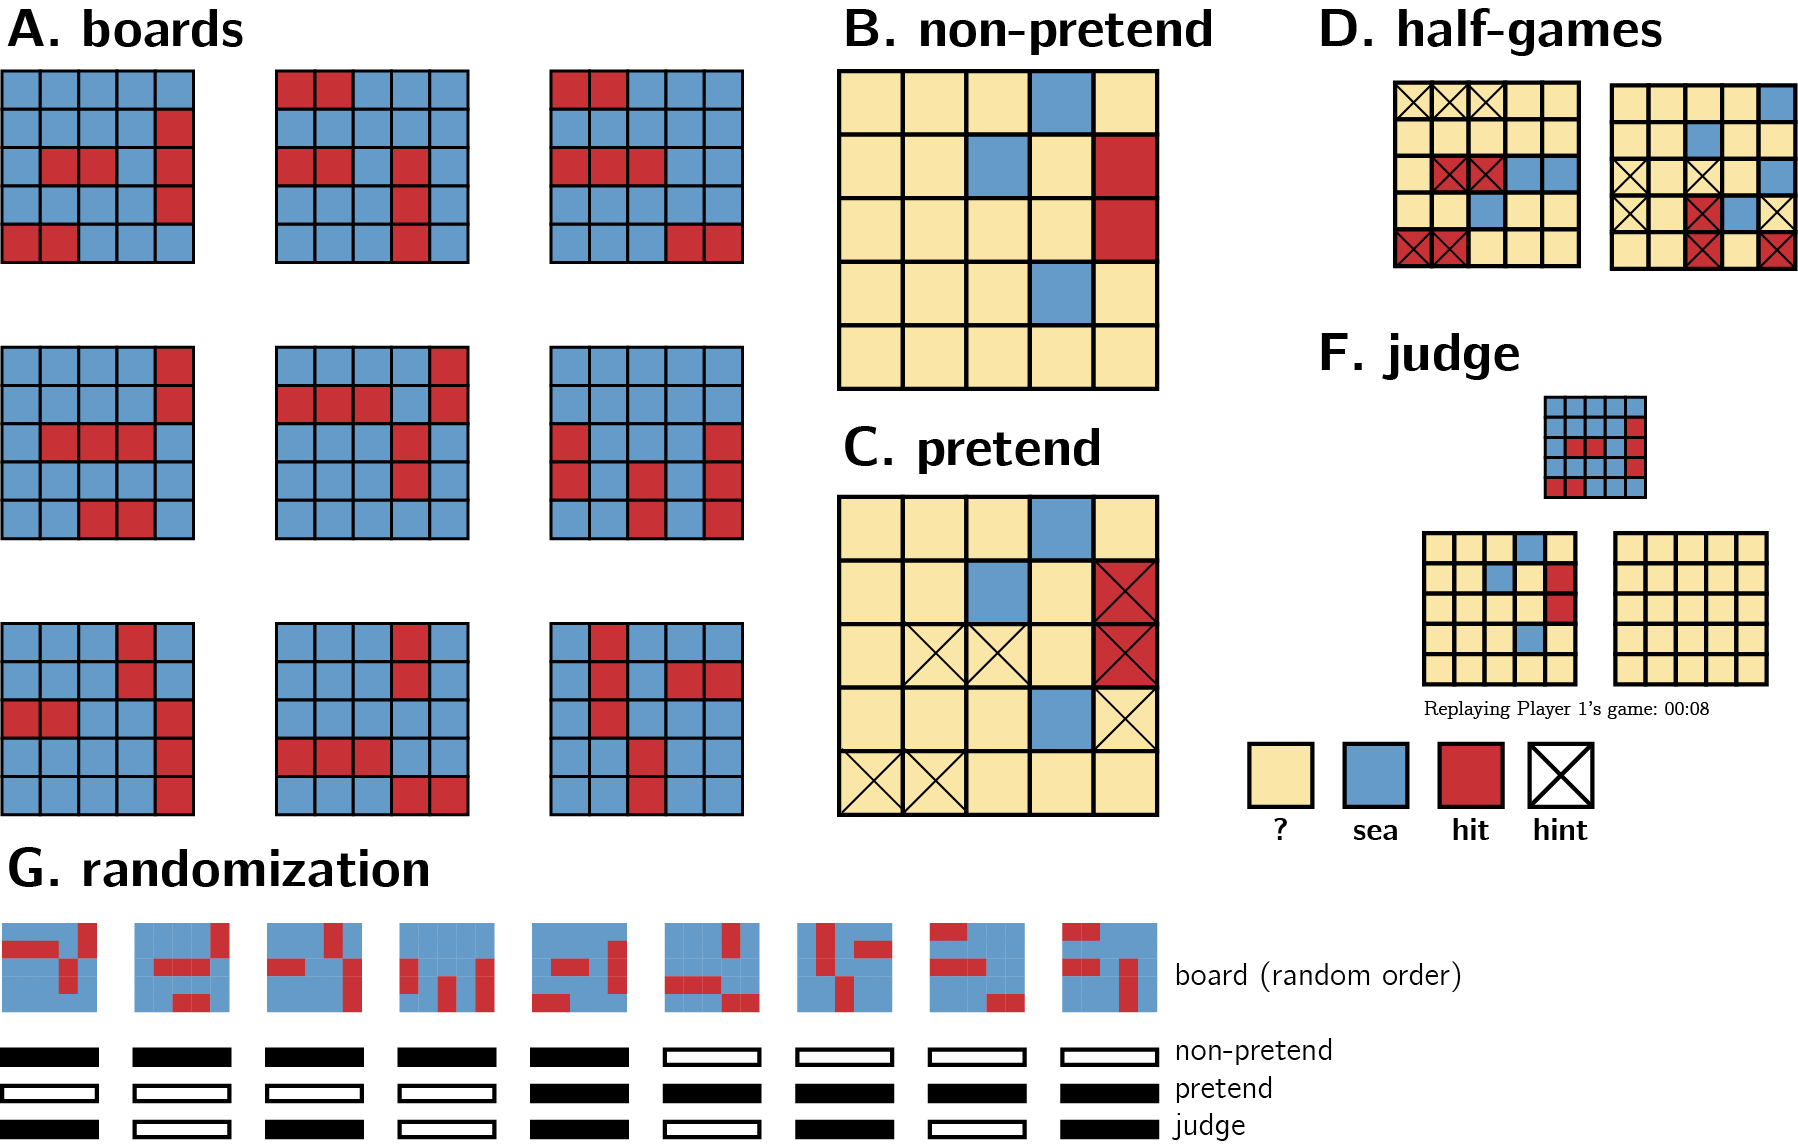
\includegraphics[width=1\linewidth]{../figures/Battleships_design} \caption[Experimental Design]{Experimental Design. See Methods for details.}\label{fig:design}
\end{figure}
\end{CodeChunk}

\hypertarget{results}{%
\section{Results}\label{results}}

We designed our analyses to explore subjects' capacity for
self-simulation under a counterfactual knowledge state, and the limits
of this capacity. We focused on where subjects clicked and when, and
asked whether this differed between pretend and non-pretend games. All
analyses were pre-registered unless otherwise specified. In our
pre-registration document, we committed to separately analyzing
participants according to whether they pretended before or after
completing a non-pretend block. Due to space limitations, and since the
results of the two groups mostly agreed, we report here the pooled
results from both groups of participants, and mention whenever we found
different results depending on block order. When directly comparing
pretend and non-pretend blocks, we perform a between-subjects comparison
using data from the first block only, i.e., pretend games from
participants who pretended in the first block and non-pretend games from
participants who played normally in the first block. We do so to ensure
that any successful pretending is not due to memory of one's own
behavior in a previous block, and that non-pretend games are not biased
by experience with the pretend block.

\hypertarget{total-number-of-clicks}{%
\subsection{Total number of clicks}\label{total-number-of-clicks}}

To sink all ships, players had to click on at least 7 and at most 25
squares. A simulated player that clicks randomly had a median total
click number of 23, and a near-optimal greedy player that consistently
selected the square with the highest objective probability of containing
a ship had a median total click number of 14. Among our players, the
median number of clicks was 16 in both pretend and non-pretend games
(see Fig. 2A).

We observed no significant difference in the number of clicks between
the two conditions (\(t(440.10) = 0.41\), \(p = .682\)). However, a
significant interaction with block order suggested that participants
made fewer clicks in the second block compared to the first, regardless
of which block was the pretend block (\(F(1, 996) = 10.59\),
\(\mathit{MSE} = 6.55\), \(p = .001\)).

In 62 pretend games from 20 players, games were completed after 7 clicks
only, without ever missing a ship. This never happened in non-pretend
games. We assumed that these participants did not follow task
instructions, and excluded them from all following analyses.

\hypertarget{game-optimality}{%
\subsection{Game optimality}\label{game-optimality}}

Pretend games were similar to non pretend games in the total number of
clicks --- but were they also similar in \emph{where} participants
clicked? More specifically, did cell selections in pretend games make
sense given the limited information those participants pretended to
have? To ask this, we approximated optimal behavior by calculating the
probability that a ship is hidden in each cell given available
information, \(p(ship(x_{i}))\), and the posterior probability that one
should click on a square, assuming a uniform prior over cells
\(P(x_{i})=\frac{p(Ship(x_i))}{\sum_{j=1}^{k}p(Ship(x_j))}\).
Critically, in modeling pretend games we did not treat hints as part of
this available information for extracting \(p(ship(x_{i}))\), because an
optimal player should ignore hints in choosing where to click next.
Given this posterior map, a rational player should choose cells where
\(P(x_{i})\) is high {[}this behavior is not strictly optimal, but
approximates optimal behavior in most cases; Audinot, Bonnet, \& Viennot
(2014), Section 3.3{]}. To quantify optimality, before each cell
selection we computed the posterior probability map for all `unknown'
cells. Then, we ranked cells from high to low according to their
posterior probability and recorded the rank of the chosen cell: a lower
rank indicating more optimal behavior.

The mean posterior rank of non-pretend cell selections was 6.44 and
significantly lower (more optimal) than that of a simulated random agent
(see Fig. 2B; 9.18, \(t(479) = -48.34\), \(p < .001\)). Pretend games
were significantly less optimal than non-pretend games (6.93;
\(t(474.06) = -6.07\), \(p < .001\)), but still more optimal than those
of a random agent (\(t(479) = -38.09\), \(p < .001\)). Critically, the
same pattern was observed when restricting analysis to cell selections
that resulted in a miss (non-pretend - pretend: \(t(469.71) = -6.30\),
\(p < .001\); pretend - random: \(t(479) = -10.26\), \(p < .001\)). In
other words, the optimality of pretend games relative to random cell
selection was not merely due to the fact that pretenders clicked on
ships more than expected by chance. Even when missing a ship, their cell
selections made sense given the limited information they pretended to
have.

\begin{CodeChunk}
\begin{figure}[tb]
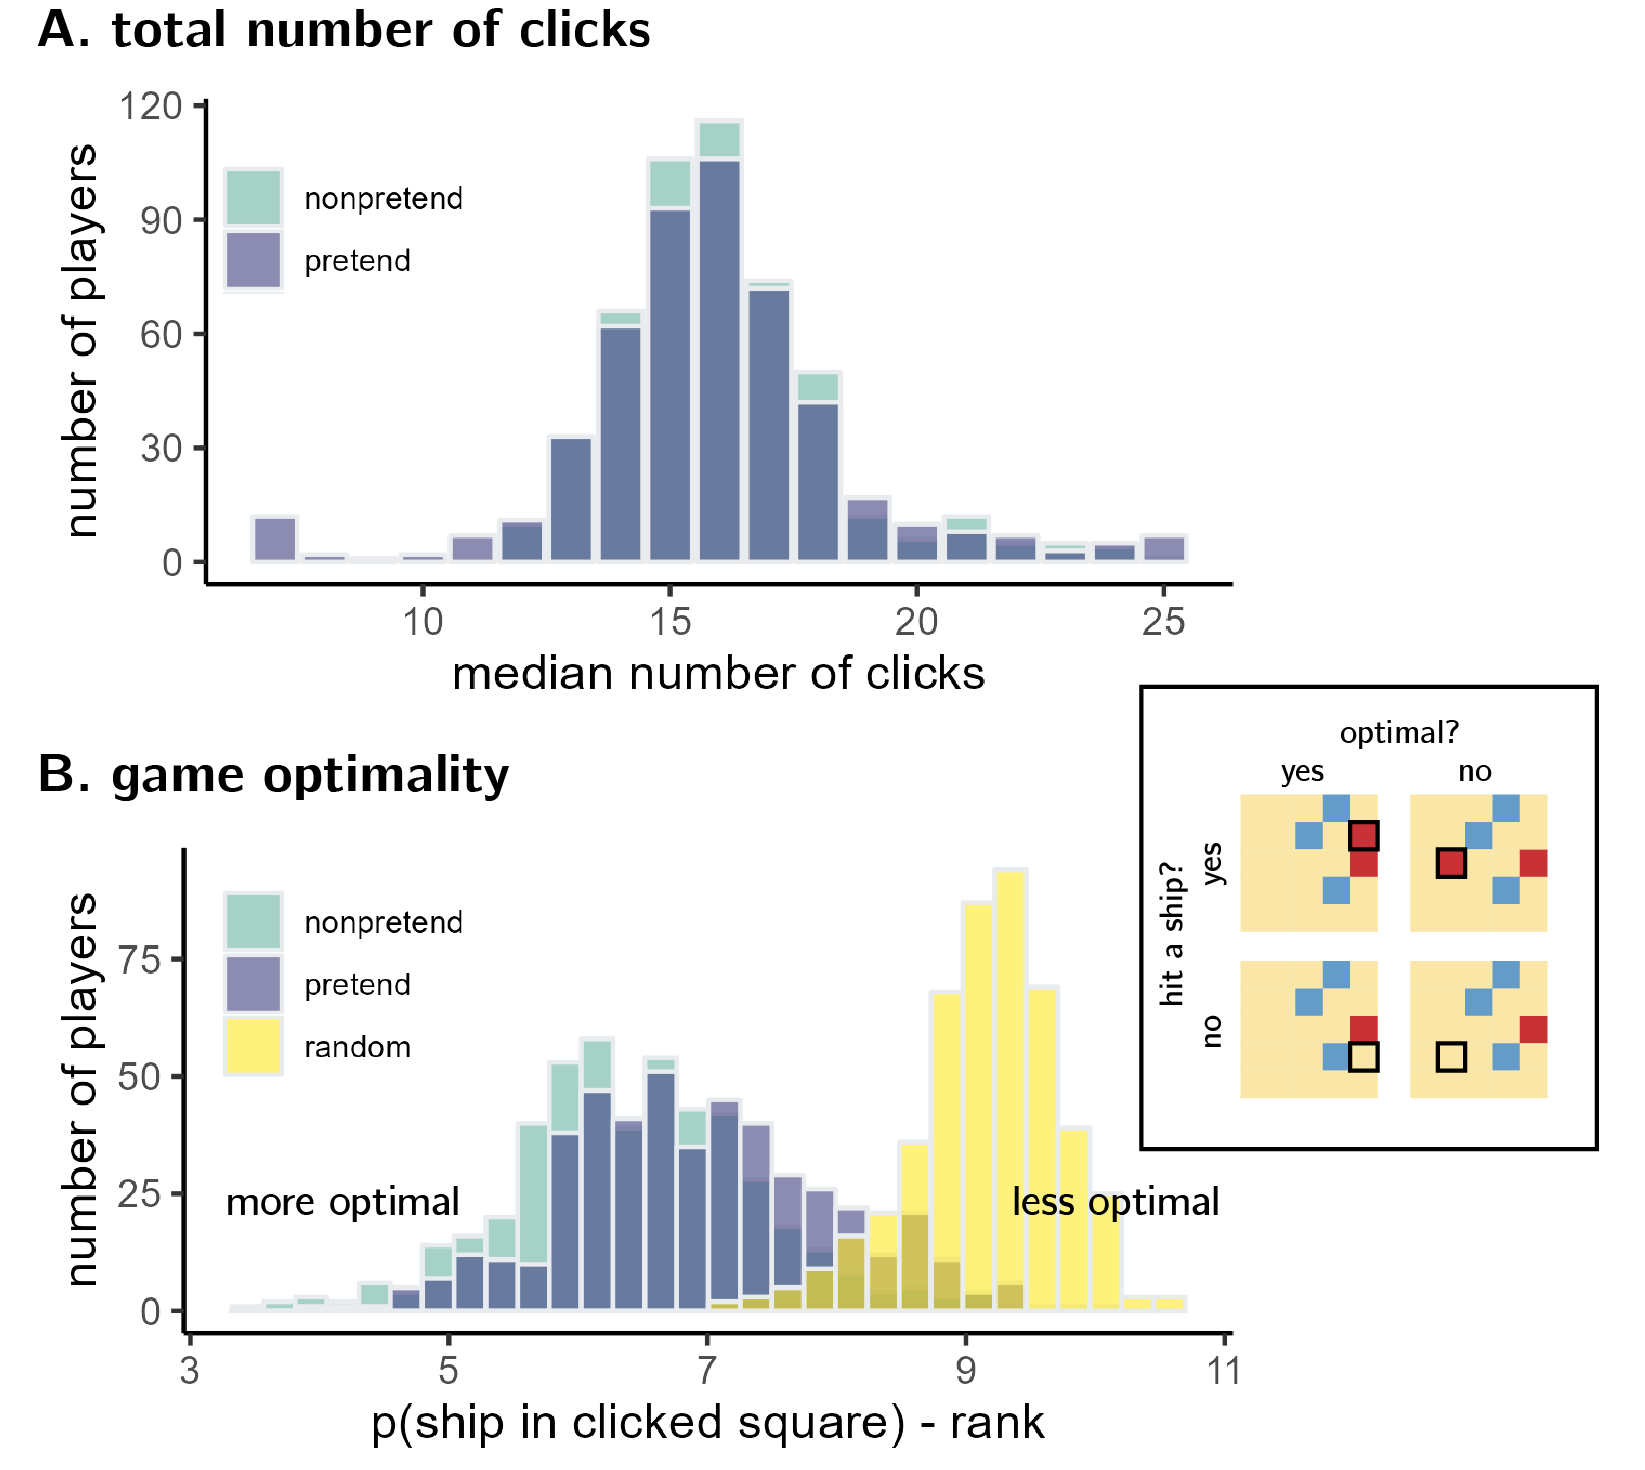
\includegraphics[width=1\linewidth]{../figures/numclicks_optimality} \caption[A]{A: The total number of clicks in pretend and non-pretend games was highly similar. B: Non-pretend games were significantly more optimal than pretend games, but both were more optimal than what is expected by random chance. Box: An illustration of the difference between success and optimality. A given click (highlighted with a black border) can reveal a ship (upper row) or not (lower row) regardless of whether the click makes sense given available information (left column) or not (right column). }\label{fig:numclick_optimality}
\end{figure}
\end{CodeChunk}

\hypertarget{response-time-analysis}{%
\subsection{Response time analysis}\label{response-time-analysis}}

In general, participants gave slower responses when pretending compared
to when playing normally. Despite the similar number of clicks per game,
the median game duration was 22.31 seconds in the non-pretend condition
and 29.23 seconds in the pretend condition, which was significantly
longer (\(t(479) = 12.68\), \(p < .001\)). This difference showed a
significant interaction with the order of conditions, such that
completing games in the first block took longer (\(F(1, 956) = 21.24\),
\(\mathit{MSE} = 243.45\), \(p < .001\), \(\hat{\eta}^2_G = .022\)).

In our instructions to pretenders, we asked them to pretend not to know
where the ships were, not only in \emph{where} they chose to click, but
also in \emph{when} they clicked. In the following set of analyses, we
identified patterns in click latency in non-pretend games, and asked
whether the same patterns are also observed in pretend games. We focused
on the effects of hitting versus missing a ship, decision uncertainty,
and ship completion.

\hypertarget{effects-of-hitting-versus-missing-a-ship}{%
\subsubsection{Effects of hitting versus missing a
ship}\label{effects-of-hitting-versus-missing-a-ship}}

In non-pretend games, players were faster by 109 ms (12\%) when hitting
compared to missing a ship (see Fig. 3A; \(t(479) = -12.37\),
\(p < .001\)). The same effect was observed in pretend games: players
were faster by 293 ms (31\%) in hits compared to misses
(\(t(233) = -11.83\), \(p < .001\); pretend first: \(t(479) = -16.23\),
\(p < .001\)). However, this difference between hits and misses was
significantly more pronounced in pretend games (\(t(314.67) = -7.45\),
\(p < .001\)).

The opposite effect was observed for a hit on the previous click:
players were slower by 182 ms (15\%) after hitting a ship
(\(t(479) = 13.39\), \(p < .001\)). This effect was also observed in
pretend games, where players were slower by 236 ms (16\%) following a
hit on the previous click (\(t(479) = 12.02\), \(p < .001\)). Again, the
absolute effect in ms was exaggerated in the pretend condition
(\(t(377.12) = 2.75\), \(p = .006\)).

\hypertarget{effects-of-decision-uncertainty}{%
\subsubsection{Effects of decision
uncertainty}\label{effects-of-decision-uncertainty}}

When playing Battleships, it is sometimes clear what the next cell
selection should be, and sometimes more difficult to decide where to
click next. To capture this notion of decision uncertainty, we
calculated the entropy of the posterior distribution over cell
selections \(H(P)=-\sum_{i=1}^{k}P(x_i) \log P(x_{i})\), where
\(P(x_{i})=\frac{p(Ship(x_i))}{\sum_{j=1}^{k}p(Ship(x_j))}\), and asked
how this measure relates to decision latency, or the time taken to click
on the next cell. \(H(P)\) is high when players need to decide between
multiple cells with a similar probability of hiding a ship, and low when
there are only a few candidates with a high probability of hiding a
ship. For every player and condition separately, we fitted a multiple
linear regression to predict decision latency based on \(H(P)\) and
\(H(P)^2\). The resulting coefficients were then subjected to a
group-level inference. The first cell selection of each game was
excluded from this analysis, because entropy was constant for the first
click.

In non-pretend games, we found no evidence for a linear relation between
decision entropy and decision latency (\(t(479) = -1.67\),
\(p = .096\)). We did however observe a block order effect, with a
significantly negative linear modulation only in the group that
pretended in the first (\(t(233) = -10.24\), \(p < .001\)), but not in
the second block (\(t(245) = -0.06\), \(p = .950\)). In pretend games
this negative relation between \(H(P)\) and click latency was
significant in both groups, as well as overall (\(t(479) = -7.42\),
\(p < .001\)).

A negative linear modulation of \(H(P)\) on decision latency is
surprising, as it suggests that participants were quicker to decide when
uncertainty was high. However, visual inspection of the RT/entropy
curves (Fig. 3B) reveals a pronounced quadratic modulation, such that in
both pretend and non-pretend games slower decision times are observed
for intermediate \(H(P)\) values of around 2. Similar to the linear
effect of \(H(P)\) on decision latency, here too a quadratic modulation
in non-pretend games was observed only in the group that pretended in
the first (\(t(233) = -13.26\), \(p < .001\)), but not in the second
block (\(t(245) = -1.33\), \(p = .184\)). Again, in pretend games this
negative quadratic relation was significant in both groups, as well as
overall (\(t(479) = -15.65\), \(p < .001\)). A between-subjects
comparison focusing on games from the first block revealed that this
negative quadratic effect was stronger in pretend, compared to
non-pretend games (\(t(363.42) = 3.46\), \(p = .001\)).

\begin{CodeChunk}
\begin{figure}[tb]
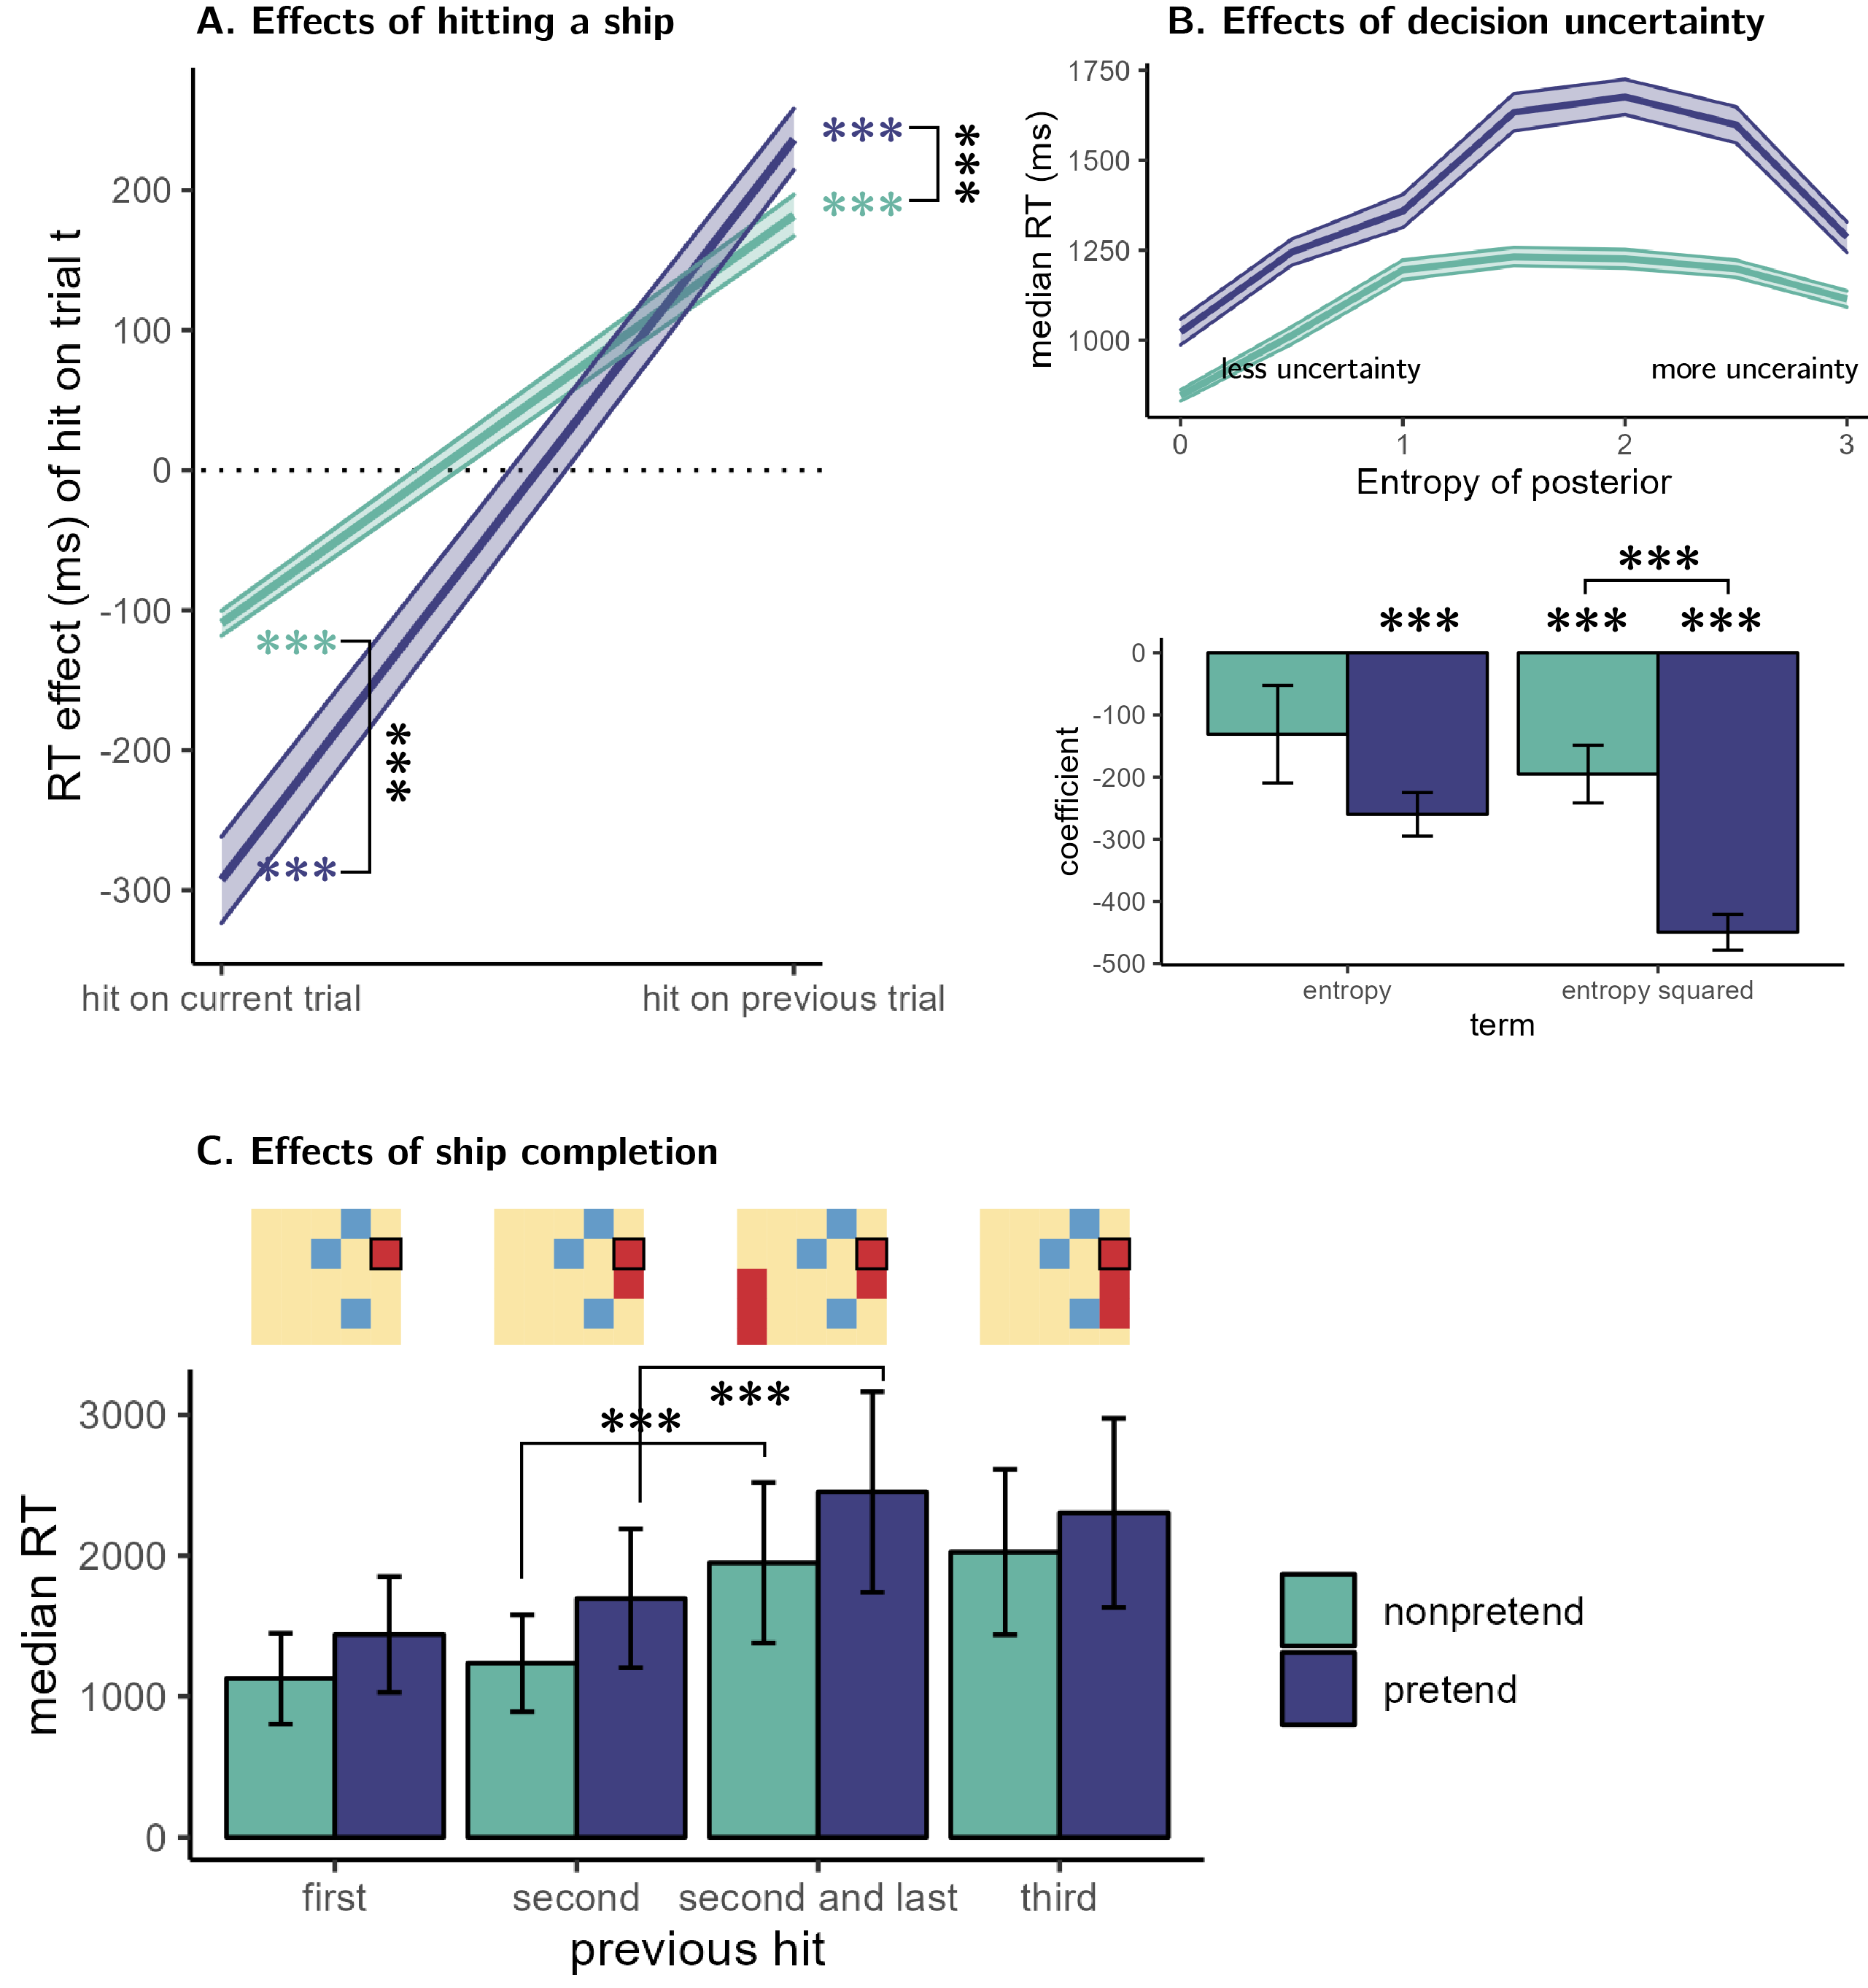
\includegraphics[width=1\linewidth]{../figures/decision_latencies} \caption[A]{A: A subtraction of decision latencies in misses versus hits in the current and previous cell selections, in pretend and non-pretend games. B. Upper panel: Effect of the entropy of the posterior distribution over cell selections (a measure of decision uncertainty) on decision latency in pretend and non-pretend games. Lower panel: mean beta coefficients for a multiple regression model, predicting decision latency from entropy and entropy squared. C: Decision latency after a hit, as a function of hit number.}\label{fig:latency}
\end{figure}
\end{CodeChunk}

\hypertarget{effects-of-ship-completion}{%
\subsection{Effects of ship
completion}\label{effects-of-ship-completion}}

The previous analyses reveal robust associations between game state and
decision latency, that are highly similar, and even exaggerated, in
pretend compared to non-pretend games. To get at subtler dynamics in a
more direct way, in a follow-up exploratory analysis we focused on
decision latencies following a hit. We categorized hits into four types:
first hit on a ship, second hit on a ship when the size-three submarine
hasn't been sunk yet, second hit on a ship when the size-three submarine
has already been sunk, and third hit on a submarine (see Fig. 3C). In
the first case, players know the ship must continue in one of the
neighboring cells. In the second case, there is a good chance the ship
continues (if this ship turns out to be a submarine). In the third and
fourth cases, it is clear that the ship is fully sunk.

In non-pretend games, participants were significantly slower to select
the next cell when they knew they had just completed a ship (categories
3 and 4) compared to when they just hit a ship, but were not sure
(category 2) or knew they had not completely sunk it (category 1;
\(t(404) = -16.82\), \(p < .001\)). Specifically, we find that
participants were slower by 728 ms to make the next cell selection after
hitting the second cell of a ship if the size-three submarine had
already been sunk (\(t(404) = 13.45\), \(p < .001\)).

Strikingly, we found the exact same pattern in pretend games. Players
were faster to make the next cell selection when they pretended to think
that the current ship might not be fully sunk (\(t(369) = -14.47\),
\(p < .001\)). This was not merely a difference between the first,
second and third hits: participants were slower by 754 ms to make the
next cell selection after hitting the second cell of a ship if the
size-three submarine had already been sunk (\(t(404) = 13.45\),
\(p < .001\)). Further analysis confirmed that this effect remained
significant when controlling for click number (\(t(404) = 11.28\),
\(p < .001\)), and when restricting the analysis to the second hit of a
ship that is in fact of size-two (\(t(366) = 3.91\), \(p < .001\)).

This last finding bears emphasizing: In both classes two and three,
pretenders \emph{knew} that they had just sunk a size-two ship, but in
the second case they \emph{pretended not to know} this fact, and this
affected their their response latency in the same way it would have been
affected had they been in a non-pretend game.

\hypertarget{half-games-1}{%
\subsection{Half-games}\label{half-games-1}}

Our optimality analysis showed that pretenders' click selections closely
resemble those of non-pretenders, at least in that they are not random,
but rather guided by where a ship might be. However, due to the high
number of possible board configurations, data from full games provide
limited opportunity to compare cell selections for specific game states.
In addition to asking, ``What guides cell selections in pretend and
non-pretend games?'', we also wanted to ask, ``Where exactly would
pretenders and non-pretenders click, given a specific board
configuration?''.

To achieve this, the sixth game in each block started not with an empty
grid, but with the contents of some cells already revealed by a previous
player. As before, pretenders also knew where the remaining ships were
hidden, but tried to play as if they only knew what was known to this
previous player. Having cell selections from 250 players for each board
configuration and condition allowed us to plot and compare the
distribution of clicks under a genuine, or pretend, knowledge state.

For example, look at Board A in Fig. 4 (upper left corner). Imagine that
you need to select your next move, knowing that exactly two size-two
patrol boats and one size-three submarine are hiding in the water. Where
would you click next? Perhaps one of the two revealed ships is the
size-three submarine. In that case you want to click on the first cell
in the third row, or on the third cell in the fifth row. Or maybe these
are the two size-two patrol boats. This would mean the submarine is
hiding in some other place, and for it not to touch sides with the boats
this must be in the first row. The hit probability map in the second
column visualizes this reasoning, by plotting the normalized probability
that a ship is hidden in different cells. As can be seen, the highest
probabilities are to the sides of the revealed ships, and in the first
row.

In the third column we plot the distribution of clicks for non-pretend
players. This distribution is in agreement with the hit probability map
(board A: \(r = .81\), 95\% CI \([.55, .93]\), \(t(16) = 5.48\),
\(p < .001\); board B: \(r = .87\), 95\% CI \([.68, .95]\),
\(t(16) = 7.01\), \(p < .001\)). Finally, in the fourth column we plot
the distribution of cell selections for pretend players. Although
noisier, this distribution is also in agreement with the hit probability
map (board A: \(r = .49\), 95\% CI \([.03, .78]\), \(t(16) = 2.27\),
\(p = .037\); board B: \(r = .73\), 95\% CI \([.40, .89]\),
\(t(16) = 4.28\), \(p = .001\)), and more importantly, with the hit
distribution of non-pretenders for the same board configuration (board
A: \(r = .63\), 95\% CI \([.31, .82]\), \(t(23) = 3.89\), \(p = .001\),
board B: \(r = .87\), 95\% CI \([.73, .94]\), \(t(23) = 8.60\),
\(p < .001\)).

\begin{CodeChunk}
\begin{figure}[tb]
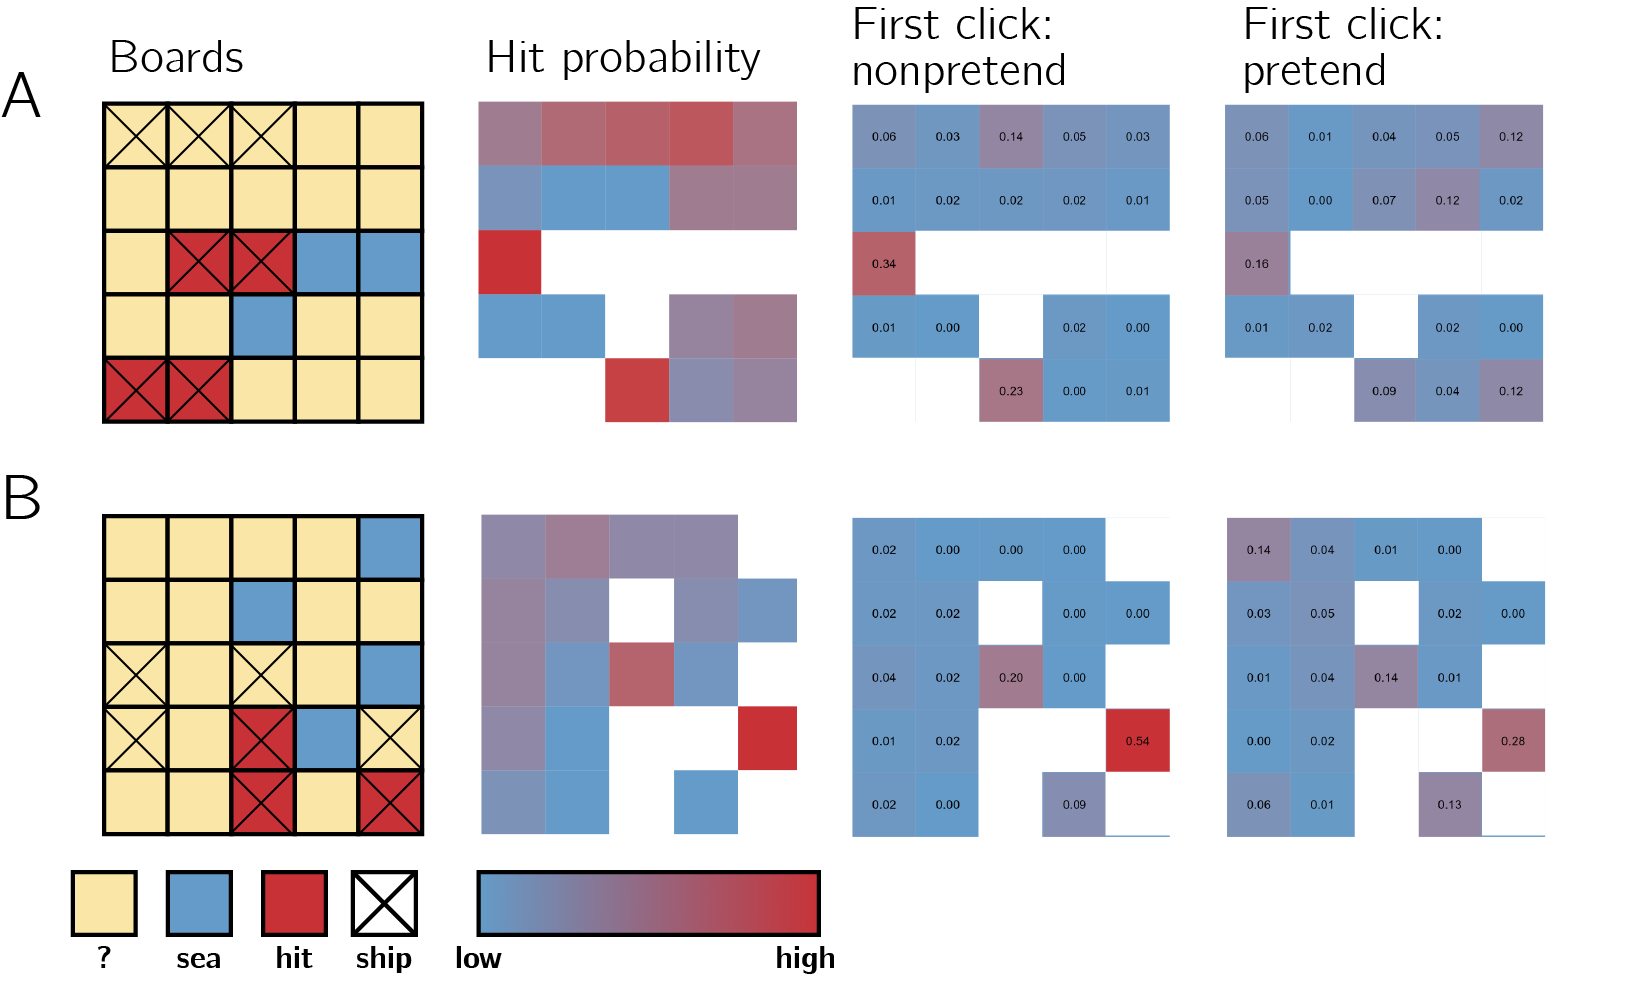
\includegraphics[width=1\linewidth]{../figures/Half_games} \caption[Half games]{Half games. First column: the two boards, as they appeared to pretenders. Second column: objective hit probability, given game state. Third and fourth columns: empirical click probabilities in non-pretend and pretend games, respectively.}\label{fig:half-games}
\end{figure}
\end{CodeChunk}

\hypertarget{judge-trials-1}{%
\subsection{Judge trials}\label{judge-trials-1}}

Despite the fact that pretenders were overall successful in mimicking
patterns of cell selection and decision latency, they also left many
clues for an independent observer to pick up on: they were slower,
displayed exaggerated effects of decision uncertainty and hit success on
response time, and were less optimal in choosing where to click next. To
illustrate, a support vector machine (SVM) algorithm reached an accuracy
level of 72\% in linearly classifying condition (pretend / non-pretend)
based on just three basic summary features: median decision latency,
game optimality score, and number of irrational clicks per game.

Despite this, participants were never significantly above chance in
judging which of the two presented games came from a pretender (mean
accuracy: 51\%; t test against 50: \(t(499) = 1.45\), \(p = .147\)).

For a subset of 288 players, one of the five boards presented in the
judging block was already presented both in the pretend and in the
non-pretend blocks. Still, even this subset of participants who had just
experienced a board both as pretenders and as non-pretenders were not
significantly above chance in telling which of two other players had
hints for this same board (mean accuracy: 55\%, \(p=.141\)).

\hypertarget{are-good-pretenders-also-better-judges}{%
\subsection{Are good pretenders also better
judges?}\label{are-good-pretenders-also-better-judges}}

The abilities to pretend and to detect pretense in others both rely on
some form of theory of mind: reasoning about counterfactual knowledge
states of oneself in the first case, and of others in the second. For
example, in scrub jays, individual birds that pilfered another bird's
caches were also more careful in hiding their own food, suggesting an
ability to project from their own experience of stealing to the behavior
of others (Emery \& Clayton, 2001). Along similar lines, we reasoned
that those participants whose pretend games better resembled the games
of genuine players would also be more accurate in detecting pretense in
others. To our surprise, this was not at all the case (\(r = -.03\),
95\% CI \([-.13, .07]\), \(t(352) = -0.56\), \(p = .573\)). Furthermore,
we find no significant correlation between participants' accuracy in
detecting the pretender and their decision optimality in pretend games
(measured as the mean rank posterior probability of their cell
selections; \(r = .01\), 95\% CI \([-.08, .10]\), \(t(478) = 0.18\),
\(p = .854\)), nor with the cost to optimality relative to non-pretend
games (\(r = .02\), 95\% CI \([-.07, .11]\), \(t(478) = 0.47\),
\(p = .641\)).

Despite our considerable sample size of 500 participants, we are
cautious in making strong claims based on the absence of a correlation
between pretense and pretense detection abilities in our sample. We
note, however, that previous developmental research has identified
weaker correlations with theory of mind measures for a tendency to
intentionally deceive another player in a game setting, compared to an
ability to detect and understand deception, potentially indicating
partly different mechanisms (Shultz \& Cloghesy, 1981).

\hypertarget{discussion}{%
\section{Discussion}\label{discussion}}

Many tasks (including writing papers for conferences) require us to
overcome the `curse of knowledge' --- the challenge of putting ourselves
in the shoes of someone who doesn't know what we know. This is just an
example of a more general fact: the ability to simulate counterfactual
knowledge states is necessary for efficient and flexible communication.
To do this, we must have an internal self-model that can generate
thoughts and behavior for hypothetical beliefs, desires, and
perceptions.

Research on Bayesian Theory of Mind provides some support for the
existence of such a model by measuring subjects' ability to infer
beliefs and desires from observed behavior, either explicitly (Baker,
Jara-Ettinger, Saxe, \& Tenenbaum, 2017; Baker, Saxe, \& Tenenbaum,
2009), or implicitly (Liu, Ullman, Tenenbaum, \& Spelke, 2017; Onishi \&
Baillargeon, 2005). Here we have put forward a complementary approach:
Asking participants to generate behavior based on a counterfactual
mental state - in this case, a counterfactual knowledge state in which a
known piece of information is unknown. Instead of relying on model
inversion (e.g., ``Which belief states would give rise to this
behavior?''), we ask participants to run the model forward, taking
beliefs and desires as input and producing behavior as output. Due to
the unconstrained space of possible behaviors in our task (cell
selections x decision latencies), successfully pretending not to know
demands a rich model of cognition, and is much harder to achieve based
on a quasi-scientific theory of mental states (Gopnik \& Wellman, 1994).

Our subjects rose to the challenge. Their pretense behavior, although
not perfect, closely resembled that of non-pretenders --- not only in
gross measures such as total number of clicks, but also in subtler
patterns of cell selection and decision latency. Our interpretation of
this finding is that participants engaged in rich and relatively
accurate counterfactual self-simulation: ``What would I have done if I
didn't have this piece of knowledge?''

An alternative interpretation is that instead of simulating a
counterfactual knowledge state, participants actively suppressed or
ignored unwanted knowledge, such that their entire cognitive machinery
was available to play the game. This does not require any self-modeling
or self-simulation, beyond the knowledge that suppressing knowledge can
be beneficial for pretending not to know something. While we cannot
fully rule out this interpretation, we think it is unlikely to explain
participants' pretense ability in our data, for two indirect reasons.
First, suppressing thoughts on demand is notoriously difficult (Wegner,
Schneider, Carter, \& White, 1987), and our first-person experience of
performing the task is that suppressing knowledge of ship locations is
hardly possible. Second, when asked how they had performed the task in a
debrief question, the responses of most participants were aligned with a
self-simulation account. In future work, we intend to more directly rule
out this knowledge-suppression hypothesis, and well as to generalize our
results to other games.

In conclusion, we propose that pretense behavior provides a unique
opportunity to directly test the richness and accuracy of subjects'
models of their own cognitive processes, and find evidence for accurate
pretending that surprisingly does not translate to an ability to detect
pretense. While more work is needed to exclude alternative explanations,
we interpret our findings as providing preliminary evidence for a
remarkable capacity for counterfactual self-simulation.

\hypertarget{references}{%
\section{References}\label{references}}

\setlength{\parindent}{-0.1in} 
\setlength{\leftskip}{0.125in}

\noindent

\hypertarget{refs}{}
\begin{CSLReferences}{1}{0}
\leavevmode\vadjust pre{\hypertarget{ref-audinot2014optimal}{}}%
Audinot, M., Bonnet, F., \& Viennot, S. (2014). Optimal strategies
against a random opponent in battleship. \emph{The 19th Game Programming
Workshop}.

\leavevmode\vadjust pre{\hypertarget{ref-baker2017rational}{}}%
Baker, C. L., Jara-Ettinger, J., Saxe, R., \& Tenenbaum, J. B. (2017).
Rational quantitative attribution of beliefs, desires and percepts in
human mentalizing. \emph{Nature Human Behaviour}, \emph{1}(4), 1--10.

\leavevmode\vadjust pre{\hypertarget{ref-baker2009action}{}}%
Baker, C. L., Saxe, R., \& Tenenbaum, J. B. (2009). Action understanding
as inverse planning. \emph{Cognition}, \emph{113}(3), 329--349.

\leavevmode\vadjust pre{\hypertarget{ref-emery2001effects}{}}%
Emery, N. J., \& Clayton, N. S. (2001). Effects of experience and social
context on prospective caching strategies by scrub jays. \emph{Nature},
\emph{414}(6862), 443--446.

\leavevmode\vadjust pre{\hypertarget{ref-emery2004mentality}{}}%
Emery, N. J., \& Clayton, N. S. (2004). The mentality of crows:
Convergent evolution of intelligence in corvids and apes.
\emph{Science}, \emph{306}(5703), 1903--1907.

\leavevmode\vadjust pre{\hypertarget{ref-frith2005theory}{}}%
Frith, C., \& Frith, U. (2005). Theory of mind. \emph{Current Biology},
\emph{15}(17), R644--R645.

\leavevmode\vadjust pre{\hypertarget{ref-gopnik1994theory}{}}%
Gopnik, A., \& Wellman, H. M. (1994). The theory theory. In \emph{An
earlier version of this chapter was presented at the society for
research in child development meeting, 1991.} Cambridge University
Press.

\leavevmode\vadjust pre{\hypertarget{ref-hall2017cooperation}{}}%
Hall, K., \& Brosnan, S. F. (2017). Cooperation and deception in
primates. \emph{Infant Behavior and Development}, \emph{48}, 38--44.

\leavevmode\vadjust pre{\hypertarget{ref-liu2017ten}{}}%
Liu, S., Ullman, T. D., Tenenbaum, J. B., \& Spelke, E. S. (2017).
Ten-month-old infants infer the value of goals from the costs of
actions. \emph{Science}, \emph{358}(6366), 1038--1041.

\leavevmode\vadjust pre{\hypertarget{ref-onishi2005fifteen}{}}%
Onishi, K. H., \& Baillargeon, R. (2005). Do 15-month-old infants
understand false beliefs? \emph{Science}, \emph{308}(5719), 255--258.

\leavevmode\vadjust pre{\hypertarget{ref-shultz1981development}{}}%
Shultz, T. R., \& Cloghesy, K. (1981). Development of recursive
awareness of intention. \emph{Developmental Psychology}, \emph{17}(4),
465.

\leavevmode\vadjust pre{\hypertarget{ref-sodian1991early}{}}%
Sodian, B., Taylor, C., Harris, P. L., \& Perner, J. (1991). Early
deception and the child's theory of mind: False trails and genuine
markers. \emph{Child Development}, \emph{62}(3), 468--483.

\leavevmode\vadjust pre{\hypertarget{ref-wegner1987paradoxical}{}}%
Wegner, D. M., Schneider, D. J., Carter, S. R., \& White, T. L. (1987).
Paradoxical effects of thought suppression. \emph{Journal of Personality
and Social Psychology}, \emph{53}(1), 5.

\leavevmode\vadjust pre{\hypertarget{ref-wimmer1983beliefs}{}}%
Wimmer, H., \& Perner, J. (1983). Beliefs about beliefs: Representation
and constraining function of wrong beliefs in young children's
understanding of deception. \emph{Cognition}, \emph{13}(1), 103--128.

\end{CSLReferences}

\bibliographystyle{apacite}


\end{document}
